\documentclass[xcolor=table]{beamer}
\usetheme{uic}
\usepackage{minted}
\usepackage{amsfonts,amsmath,oldgerm,algorithmic,algorithm}
\usepackage[font=small,labelfont=bf]{caption} % Required for specifying captions to tables and figures
\usepackage{tcolorbox}
\tcbuselibrary{listings,skins}
\usepackage{alltt,xcolor}
\usepackage{hyperref}
\usepackage{comment}
\usepackage{amsthm}
\usepackage[spanish]{babel}


\lstdefinestyle{mystyle}{
language=C
}

\newtcblisting{mylisting}[2][]{
    arc=0pt, outer arc=0pt,
    listing only, 
    listing style=mystyle,
    title=#2,
    #1
}


\newcommand{\hrefcol}[2]{\textcolor{uihteal}{\href{#1}{#2}}}
\newcommand{\testcolor}[1]{\colorbox{#1}{\textcolor{#1}{test}}~\texttt{#1}}

% Please see Section 18.1 of Beamer User Guide for all the options \usefonttheme provides
\usefonttheme[onlymath]{serif}
% \usefonttheme{serif} % use this if you would like Serif font throughout (and not just for math)

\title{Fundamentos de Inteligencia Artificial}
\titlebackground{images/etsiinformatica3.jpeg}
% an asterisk will split the background:
% \titlebackground*{images/uic_seo.jpg}
\subtitle{Búsquedas No informadas}

\author{\href{mailto:jmmontes@uma.es}{José A. Montenegro}}
\date{\today}

%https://aima.cs.berkeley.edu/algorithms.pdf


\begin{document}

\newtheorem{mydef}{Definición}[section] % Añade [section] para que se reinicie en cada sección
\maketitle

% default is no footline, but page numbers are incredibly useful for the audience to ask questions later
\footlinecolor{uicblue}

%%%%%%%%%%%%%%%%%%%%%%%%%%%%%%%%%%%%%%%%%%%%%%%%%%%
%%%%%%%%%%%%%%%%%%%%%%%%%%%%%%%%%%%%%%%%%%%%%%%%%%%
%%%%%%%%%%%%%%%%%%%%%%%%%%%%%%%%%%%%%%%%%%%%%%%%%%%
%%%%%%%%%%%%%%%%%%%%%%%%%%%%%%%%%%%%%%%%%%%%%%%%%%%
%%%%%%%%%%%%%%%%%%%%%%%%%%%%%%%%%%%%%%%%%%%%%%%%%%%
%%%%%%%%%%%%%%%%%%%%%%%%%%%%%%%%%%%%%%%%%%%%%%%%%%%


%%%%%%%%%%%%%%%%%%%%%%%%%%%%%%%%%%%%%%%%%%%%%%%%%%%
%%%%%%%%%%%%%%%%%%%%%%%%%%%%%%%%%%%%%%%%%%%%%%%%%%%
%%%%%%%%%%%%%%%%%%%%%%%%%%%%%%%%%%%%%%%%%%%%%%%%%%%
%%%%%%%%%%%%%%%%%%%%%%%%%%%%%%%%%%%%%%%%%%%%%%%%%%%
%%%%%%%%%%%%%%%%%%%%%%%%%%%%%%%%%%%%%%%%%%%%%%%%%%%
%%%%%%%%%%%%%%%%%%%%%%%%%%%%%%%%%%%%%%%%%%%%%%%%%%%


\begin{frame}{Contenido}
\tableofcontents
\end{frame}

%%%%%%%%%%%%%%%%%%%%%%%%%%%%%%%%
%%%%%%%%%%%%%%%%%%%%%%%%%%%%%%%%
%SECCION %%%%%%%%%%%%%%%%%%%%%%%%%%%%%%%
%%%%%%%%%%%%%%%%%%%%%%%%%%%%%%%%
%%%%%%%%%%%%%%%%%%%%%% 

\begin{chapter}[images/etsiinformatica4.png]{uicblue}{Búsqueda de Soluciones Informadas}
\end{chapter}

\section{Búsqueda de Soluciones Informadas}
%%%%%%%%%%%%%%%%%%%%%%%%%%%%%%%%
%%%%%%%%%%%%%%%%%%%%%%%%%%%%%%%%
%%%%%%%%%%%%%%%%%%%%%%%%%%%%%%%%

%%%%%%%%%%%%%%%%%%%%%%%%%%%%%%%%
%%%%%%%%%%%%%%%%%%%%%%%%%%%%%%%%


%%%%%%%%%%%%%%%%%%%%%%%%%%%%%%%%

\begin{frame} \frametitle{Búsquedas informadas} \small
\begin{itemize}
\item Estrategias de búsqueda informada puede encontrar soluciones de manera más eficiente que una estrategia no informada.

\item Selecciona un nodo para la expansión basada en una función de evaluación f(n).

\begin{itemize}
\item Normalmente se expande el nodo con la evaluación más baja.
\end{itemize}

\item \textbf{Función heurística h(n)}, forma más común de transmitir el conocimiento adicional del problema al algoritmo de búsqueda.


\begin{itemize}
\item coste estimado del camino más barato desde el nodo n a un nodo objetivo.
\end{itemize}

\end{itemize}

\end{frame} 

%%%%%%%%%%%%%%%%%%%%%%%%%%%%%%%%

\begin{frame} \frametitle{Algoritmo} \small

\begin{columns}

\begin{column}{0.5\textwidth}  


\begin{figure}
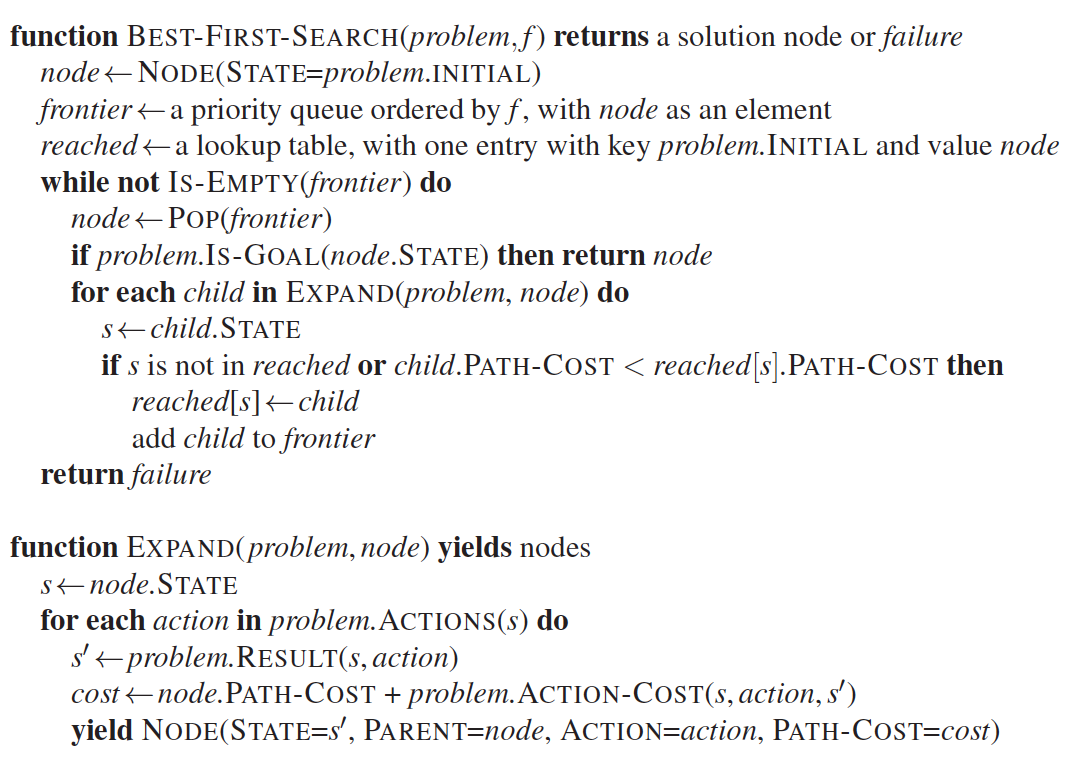
\includegraphics[scale=0.35]{./img/BFA}
\end{figure}

\end{column}

\begin{column}{0.5\textwidth}\scriptsize

Este es un algoritmo genérico en el cual elegimos un nodo, n, con el menor valor de una función de evaluación, f(n).

En los algoritmos de búsqueda se utilizan tres tipos de colas:

\begin{itemize}
    \item \textbf{Cola de prioridad} - Una cola de prioridad selecciona primero el nodo con el coste mínimo según una función de evaluación, f (n) .
    
        \item \textbf{Cola FIFO} - Una cola FIFO o cola del primero que entra es el primero que sale. Corresponde con la implementación \textbf{búsqueda ampitud}.
    \item \textbf{Cola LIFO} - Una cola LIFO o cola de último en entrar primero en salir (también conocida como pila) saca primero el nodo añadido más recientemente. Corresponde con la implementación \textbf{búsqueda profundidad}.
    
\end{itemize}


\end{column}

\end{columns}



\end{frame} 

%%%%%%%%%%%%%%%%%%%%%%%%%%%%%%%%

\begin{frame} \frametitle{Ejemplo Mapa Rumanía} \small


\begin{columns}

\begin{column}{0.6\textwidth}  
\begin{description}
\item[Estados]: Ciudades mapa
\item[Estado Inicial]: In(Arad)
\item[Función Sucesor]: Result(In(Arad),Go(Zerid))=In(Zerid)
\item[Acciones]: \{Go(Sibiu),Go(Timisora),Go(Zerind)\}
\item[Objetivo]: In(Bucharest)
\item[Coste Camin]: ver mapa
\end{description}
\end{column}

\begin{column}{0.4\textwidth}\scriptsize

\begin{figure}
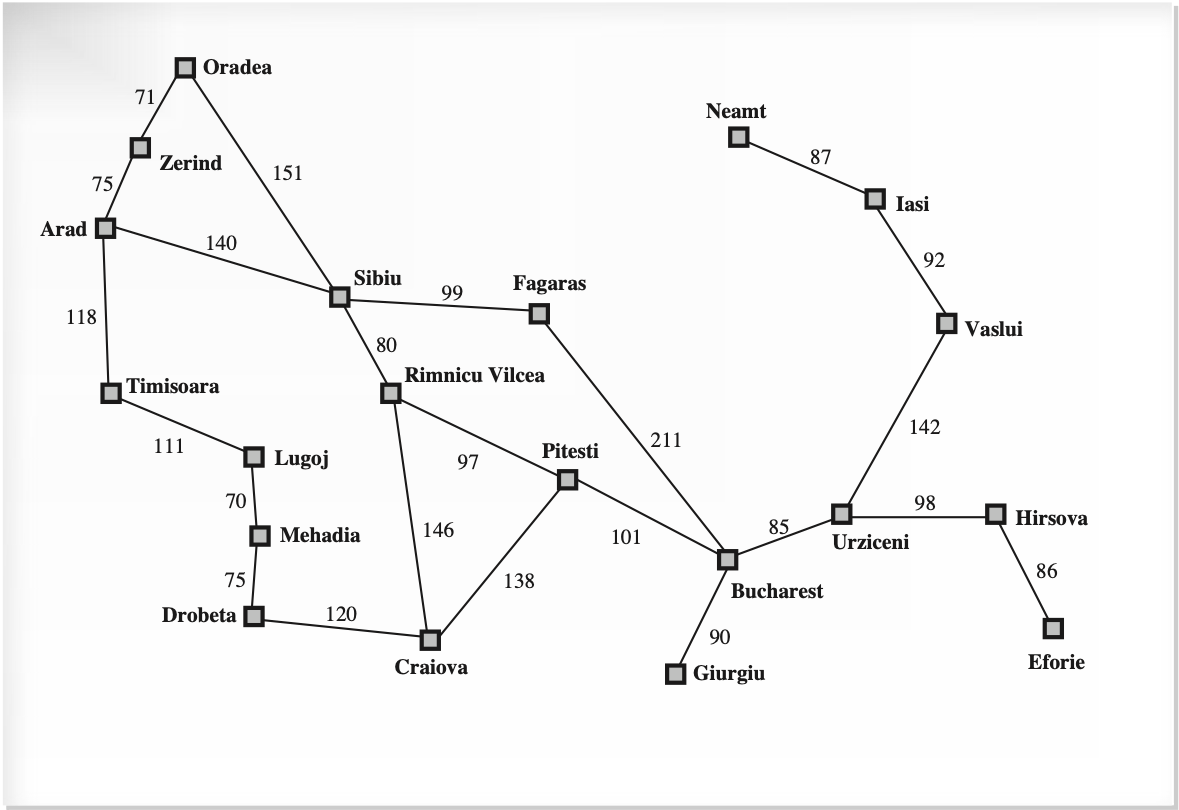
\includegraphics[scale=0.3]{./img/Rumania}
\end{figure}
\end{column}

\end{columns}

\end{frame} 



%%%%%%%%%%%%%%%%%%%%%%%%%%%%%%%%

\begin{frame} \frametitle{Ejemplo Mapa Rumanía} \small

\begin{figure}
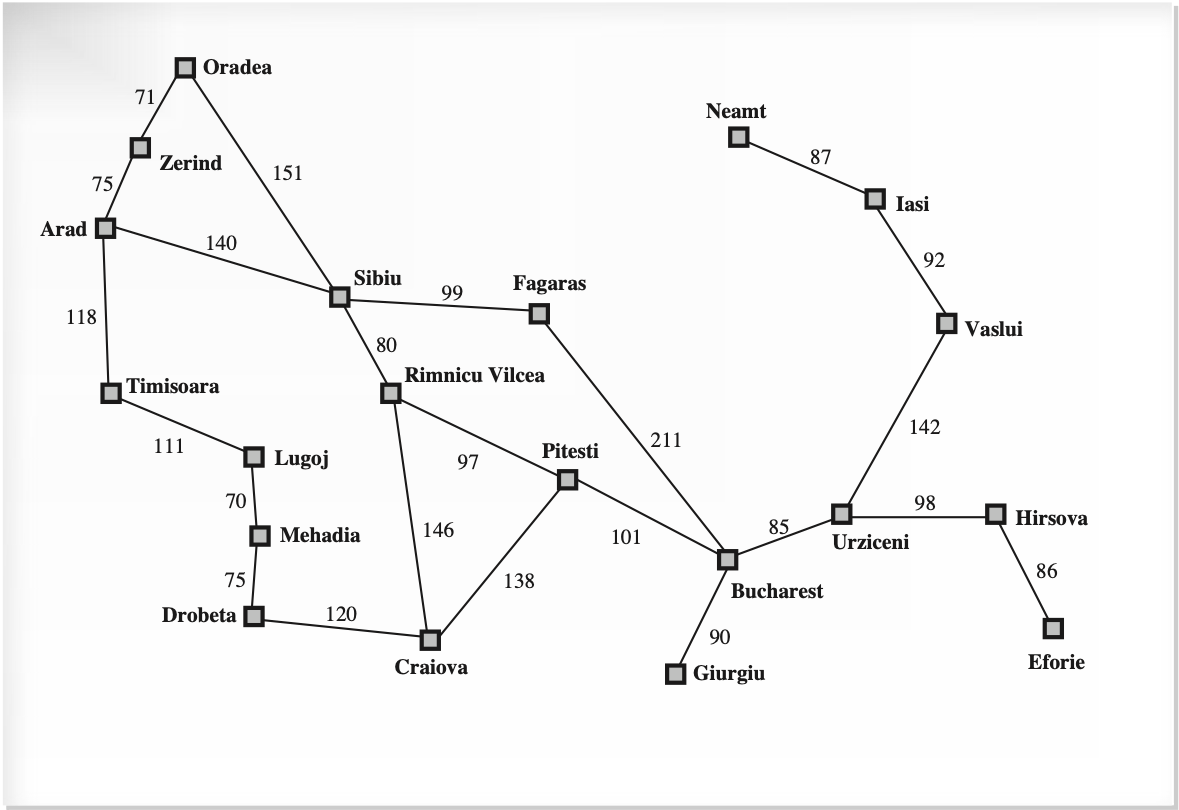
\includegraphics[scale=0.5]{./img/Rumania}
\end{figure}

\end{frame} 

%%%%%%%%%%%%%%%%%%%%%%%%%%%%%%%%
%%%%%%%%%%%%%%%%%%%%%%%%%%%%%%%%
\section{Algoritmo voraz}
\begin{chapter}[images/etsiinformatica4.png]{uicblue}{Algoritmo voraz}
\end{chapter}
%%%%%%%%%%%%%%%%%%%%%%%%%%%%%%%%
%%%%%%%%%%%%%%%%%%%%%%%%%%%%%%%%
%%%%%%%%%%%%%%%%%%%%%%%%%%%%%%%%

\begin{frame} \frametitle{Algoritmo voraz (greedy)} \footnotesize

\begin{itemize}
\item Expandir nodo más cercano al objetivo, basándose que conduce rápidamente a una solución.
\begin{itemize}
\item Función de evaluación f(n) = h(n).
\end{itemize}
\item Ejemplo h = Distancia en línea recta dos ciudades.
\begin{figure}
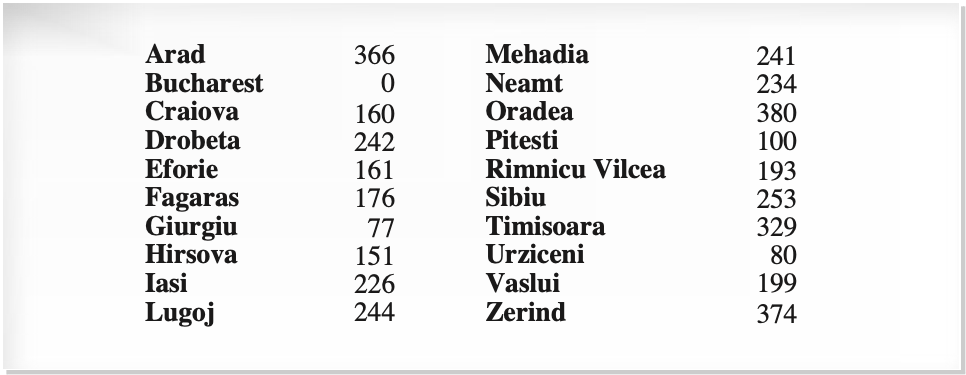
\includegraphics[scale=0.33]{./img/heuristica}
\end{figure}

\item Algoritmo no óptimo y completo en espacio de estados finitos pero no en espacio de estados infinitos.

\item La complejidad espacial y temporal en el peor caso es  O(|V|). Siendo |V| el número de vértices. 

\begin{itemize}\footnotesize
\item Una buena función heurística puede reducir la complejidad sustancialmente a  O(bm). Siendo b el factor de ramificación y  m la máxima profundidad del árbol de búsqueda.
\end{itemize}

\end{itemize}





\end{frame} 

%%%%%%%%%%%%%%%%%%%%%%%%%%%%%%%%


%%%%%%%%%%%%%%%%%%%%%%%%%%%%%%%%

\begin{frame} \frametitle{Algoritmo voraz (greedy)} \small

\begin{figure}
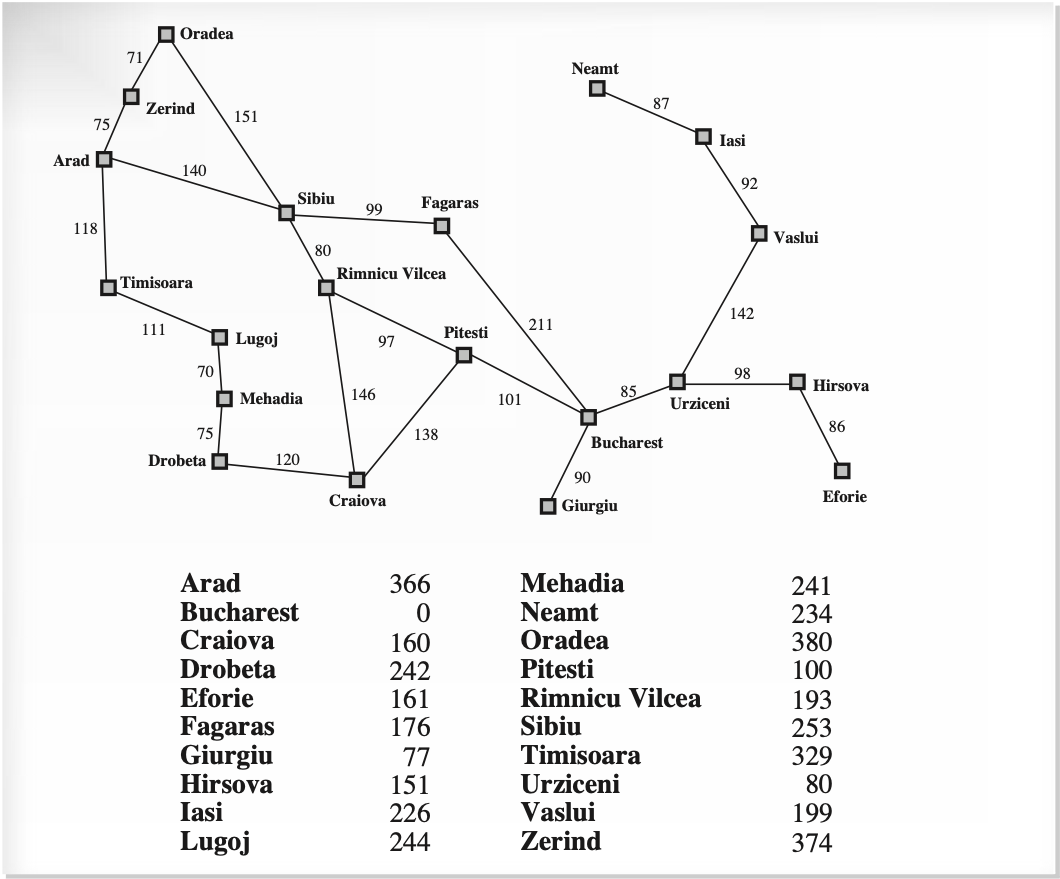
\includegraphics[scale=0.4]{./img/Mapa&Heuristica}
\end{figure}

\end{frame} 

%%%%%%%%%%%%%%%%%%%%%%%%%%%%%%%%

\begin{frame} \frametitle{Algoritmo voraz (greedy)} \small

\begin{figure}
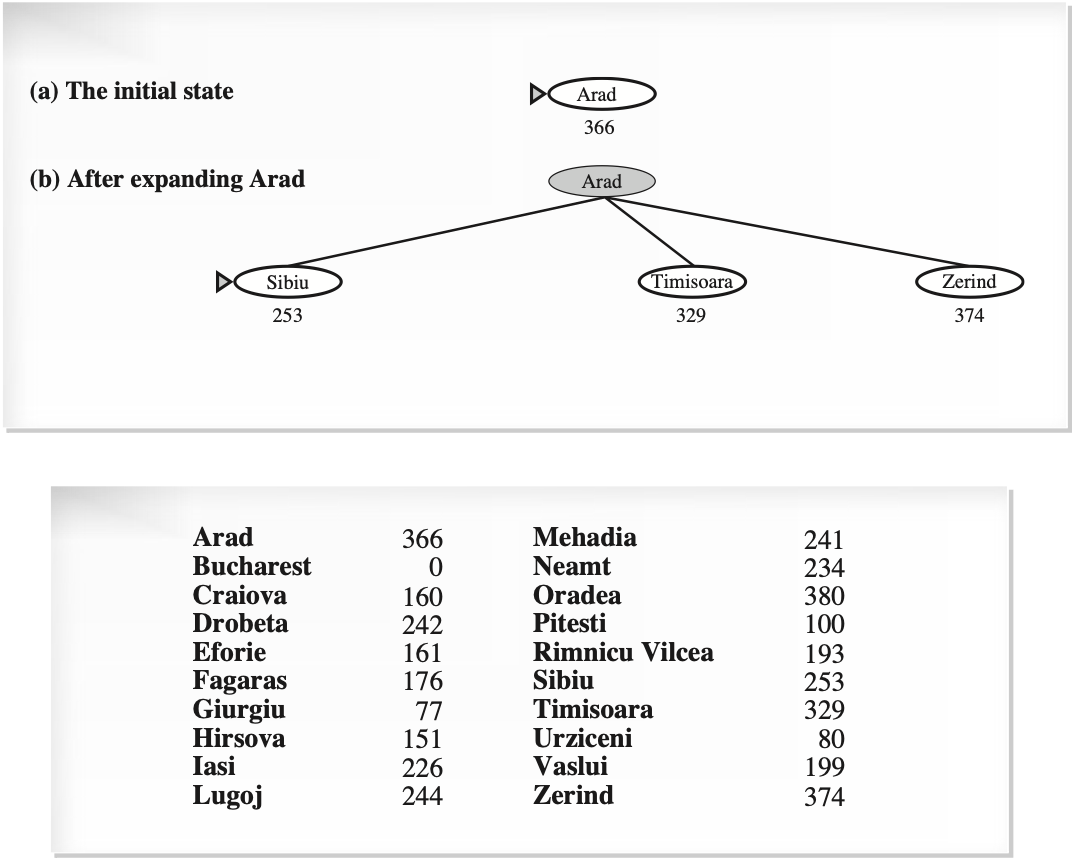
\includegraphics[scale=0.39]{./img/greedy1}
\end{figure}

\end{frame} 

%%%%%%%%%%%%%%%%%%%%%%%%%%%%%%%%

\begin{frame} \frametitle{Algoritmo voraz (greedy)} \small

\begin{figure}
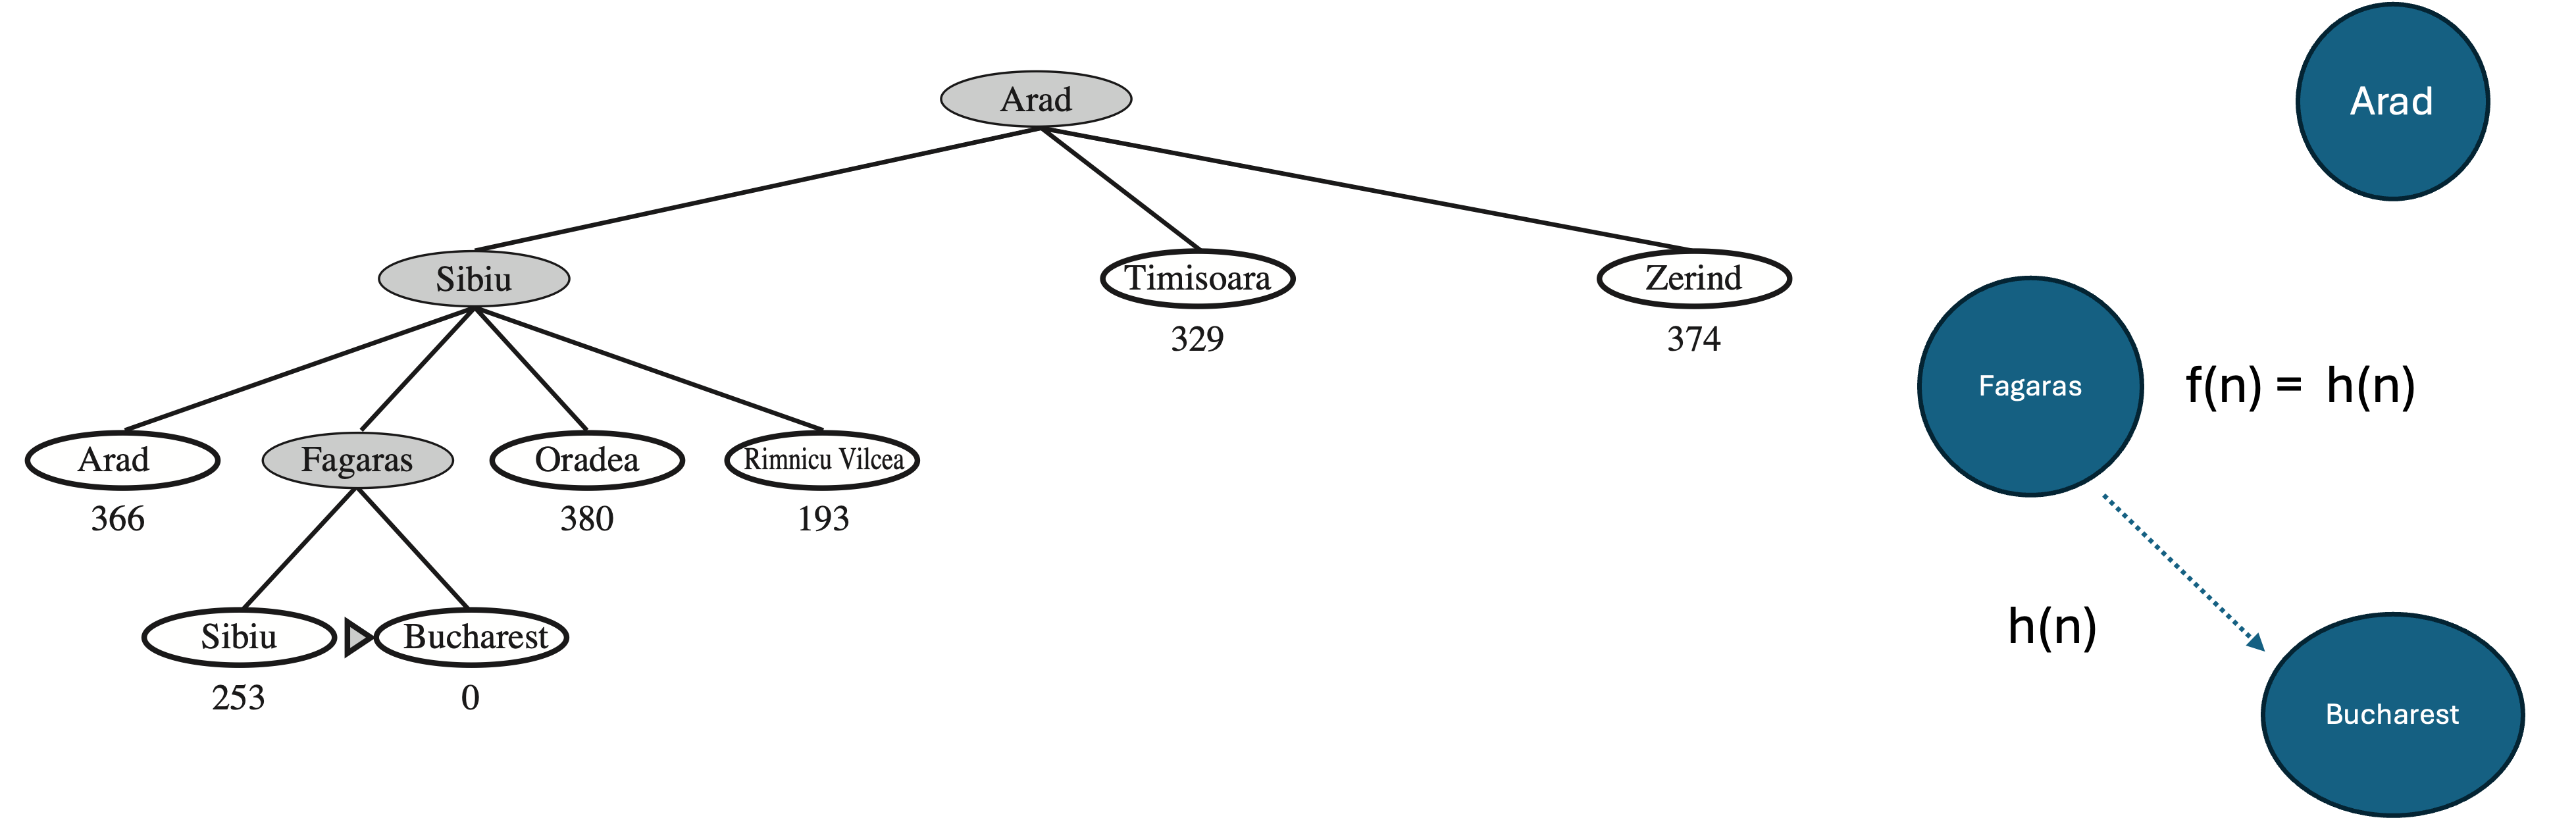
\includegraphics[scale=0.4]{./img/Gfn}
\end{figure}

\end{frame} 
%%%%%%%%%%%%%%%%%%%%%%%%%%%%%%%%

\begin{frame} \frametitle{Algoritmo voraz (greedy)} \small

\begin{figure}
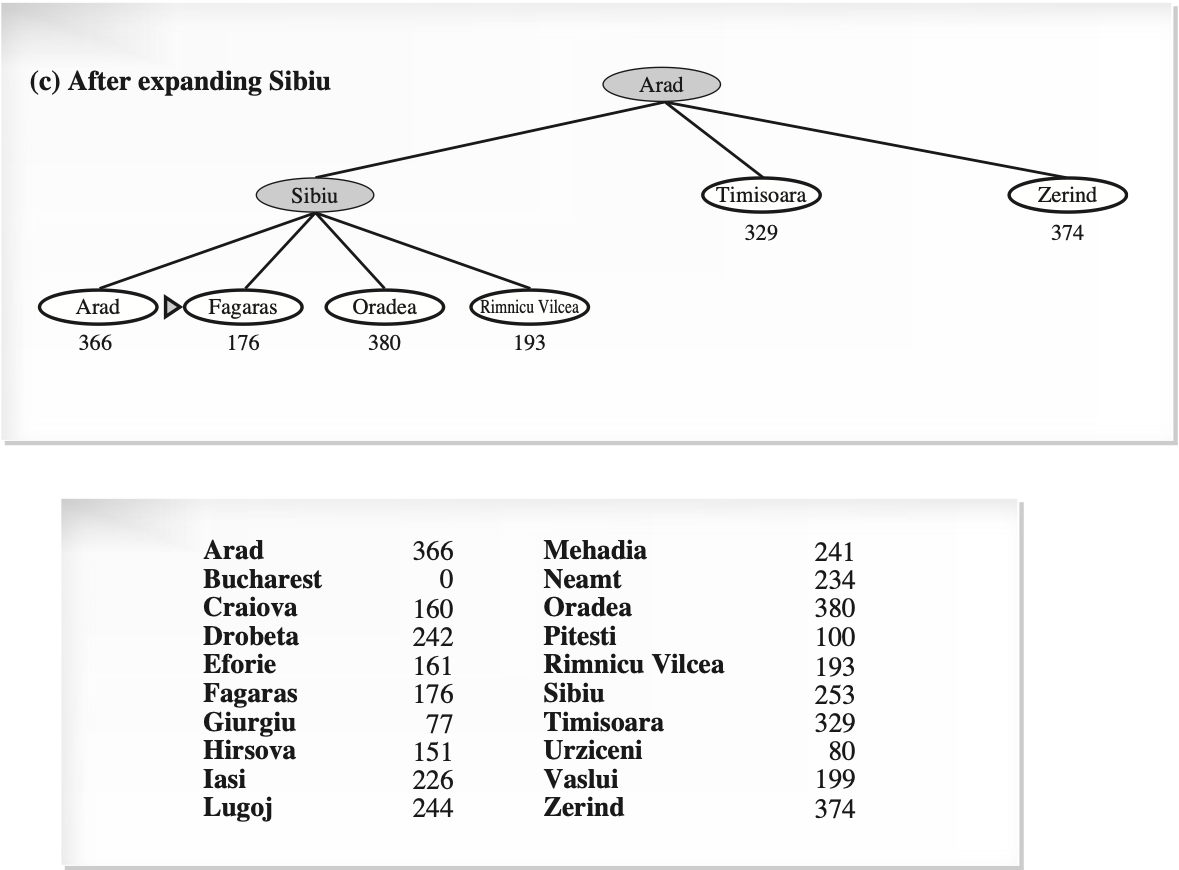
\includegraphics[scale=0.4]{./img/greedy2}
\end{figure}

\end{frame} 

%%%%%%%%%%%%%%%%%%%%%%%%%%%%%%%%

\begin{frame} \frametitle{Algoritmo voraz (greedy)} \small

\begin{figure}
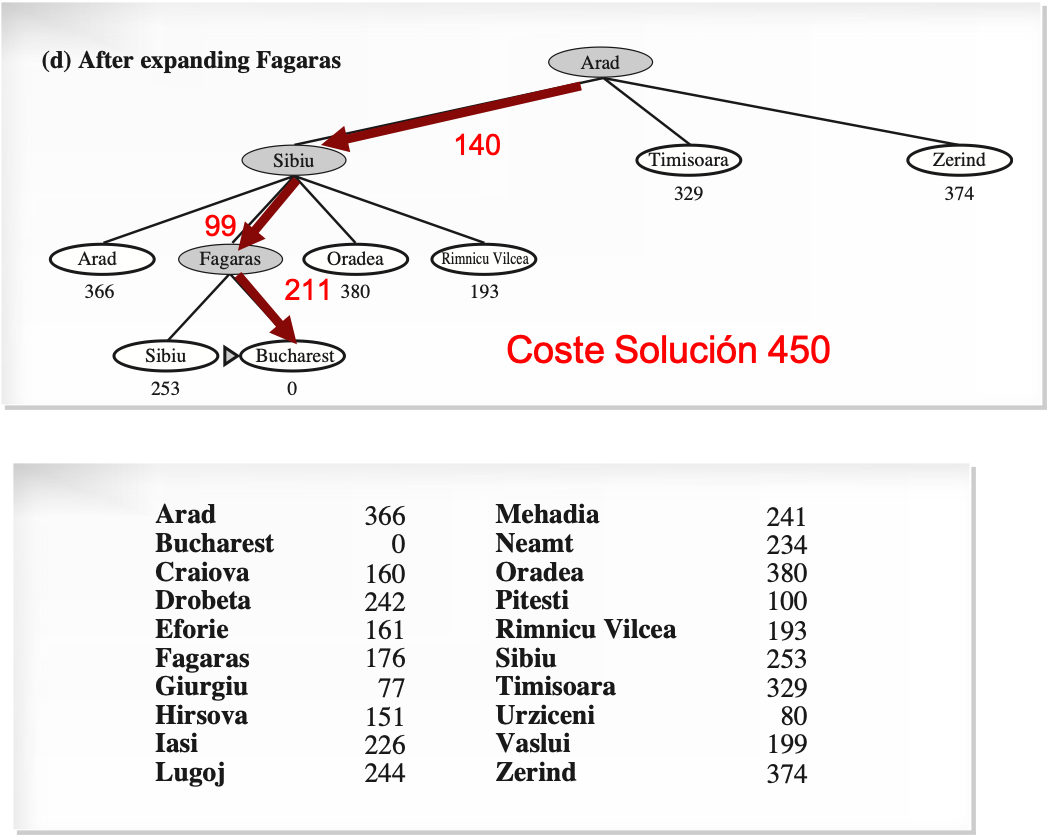
\includegraphics[scale=0.4]{./img/greedy3}
\end{figure}

\end{frame} 

%%%%%%%%%%%%%%%%%%%%%%%%%%%%%%%%
\begin{frame}  \frametitle{Ejecución greedy }\footnotesize  

\begin{table}[]
\begin{tabular}{|l|l|l|l|}
\hline
\rowcolor[HTML]{C0C0C0} 
\textbf{Nodo seleccionado}  & \textbf{Sucesor}           & \textbf{h=f}               & \textbf{Orden en que se han cerrado} \\ \hline
\textbf{Arad}      & Zerind            & 374         &           \\ \hline
-                  & Timisoara         & 329        &            \\ \hline
-                  & Sibiu             & 253         & (1)       \\ \hline\hline

\textbf{Sibiu}     & Fagaras           & 176   & (2)          \\ \hline
-                  & Oradea            & 380  &                \\ \hline
                   & Rimmicu           & 193  &             \\ \hline\hline

\textbf{Fagaras}   & Sibiu             & -                   & cerrado                     \\ \hline
-                  & Bucharest         & 0    & (3)           \\ \hline\hline
\textbf{Bucharest} & \textbf{Solución Problema} &                     &                             \\ \hline
\end{tabular}
\end{table}

\end{frame} 

%%%%%%%%%%%%%%%%%%%%%%%%%%%%%%%%
%%%%%%%%%%%%%%%%%%%%%%%%%%%%%%%%
\section{Búsqueda A*}
\begin{chapter}[images/etsiinformatica4.png]{uicblue}{Búsqueda $A^*$}
\end{chapter}

%%%%%%%%%%%%%%%%%%%%%%%%%%%%%%%%

\begin{frame} \frametitle{Búsqueda $A^*$} \footnotesize

\begin{itemize}
\item Evalúa los nodos combinando g(n), el coste para alcanzar el nodo, y h(n), el coste de ir al nodo objetivo:

\begin{itemize}
\item f(n)=g(n)+h(n)

\end{itemize}
\item $A^*$ es óptima si h(n) es una heurística \textbf{admisible}, es decir, h(n) nunca sobreestime el coste de alcanzar el objetivo. 


\begin{itemize}\footnotesize
\item Diremos que una función heurística h es admisible siempre que se cumpla que su
valor en cada nodo sea menor o igual que el valor del coste real del camino que nos falta por recorrer hasta la solución, formalmente:
$\forall n \; 0 \leq  h(n) \leq h{^*}(n)$

\end{itemize}

\end{itemize}




\begin{figure}
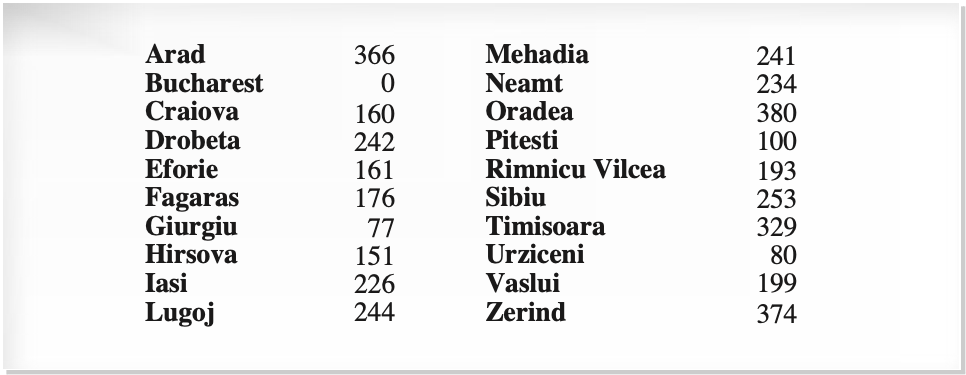
\includegraphics[scale=0.35]{./img/heuristica}
\end{figure}

\end{frame} 


%%%%%%%%%%%%%%%%%%%%%%%%%%%%%%%%
%%%%%%%%%%%%%%%%%%%%%%%%%%%%%%%%

\begin{frame} \frametitle{Ejemplo Búsqueda $A^*$} \small

\begin{figure}
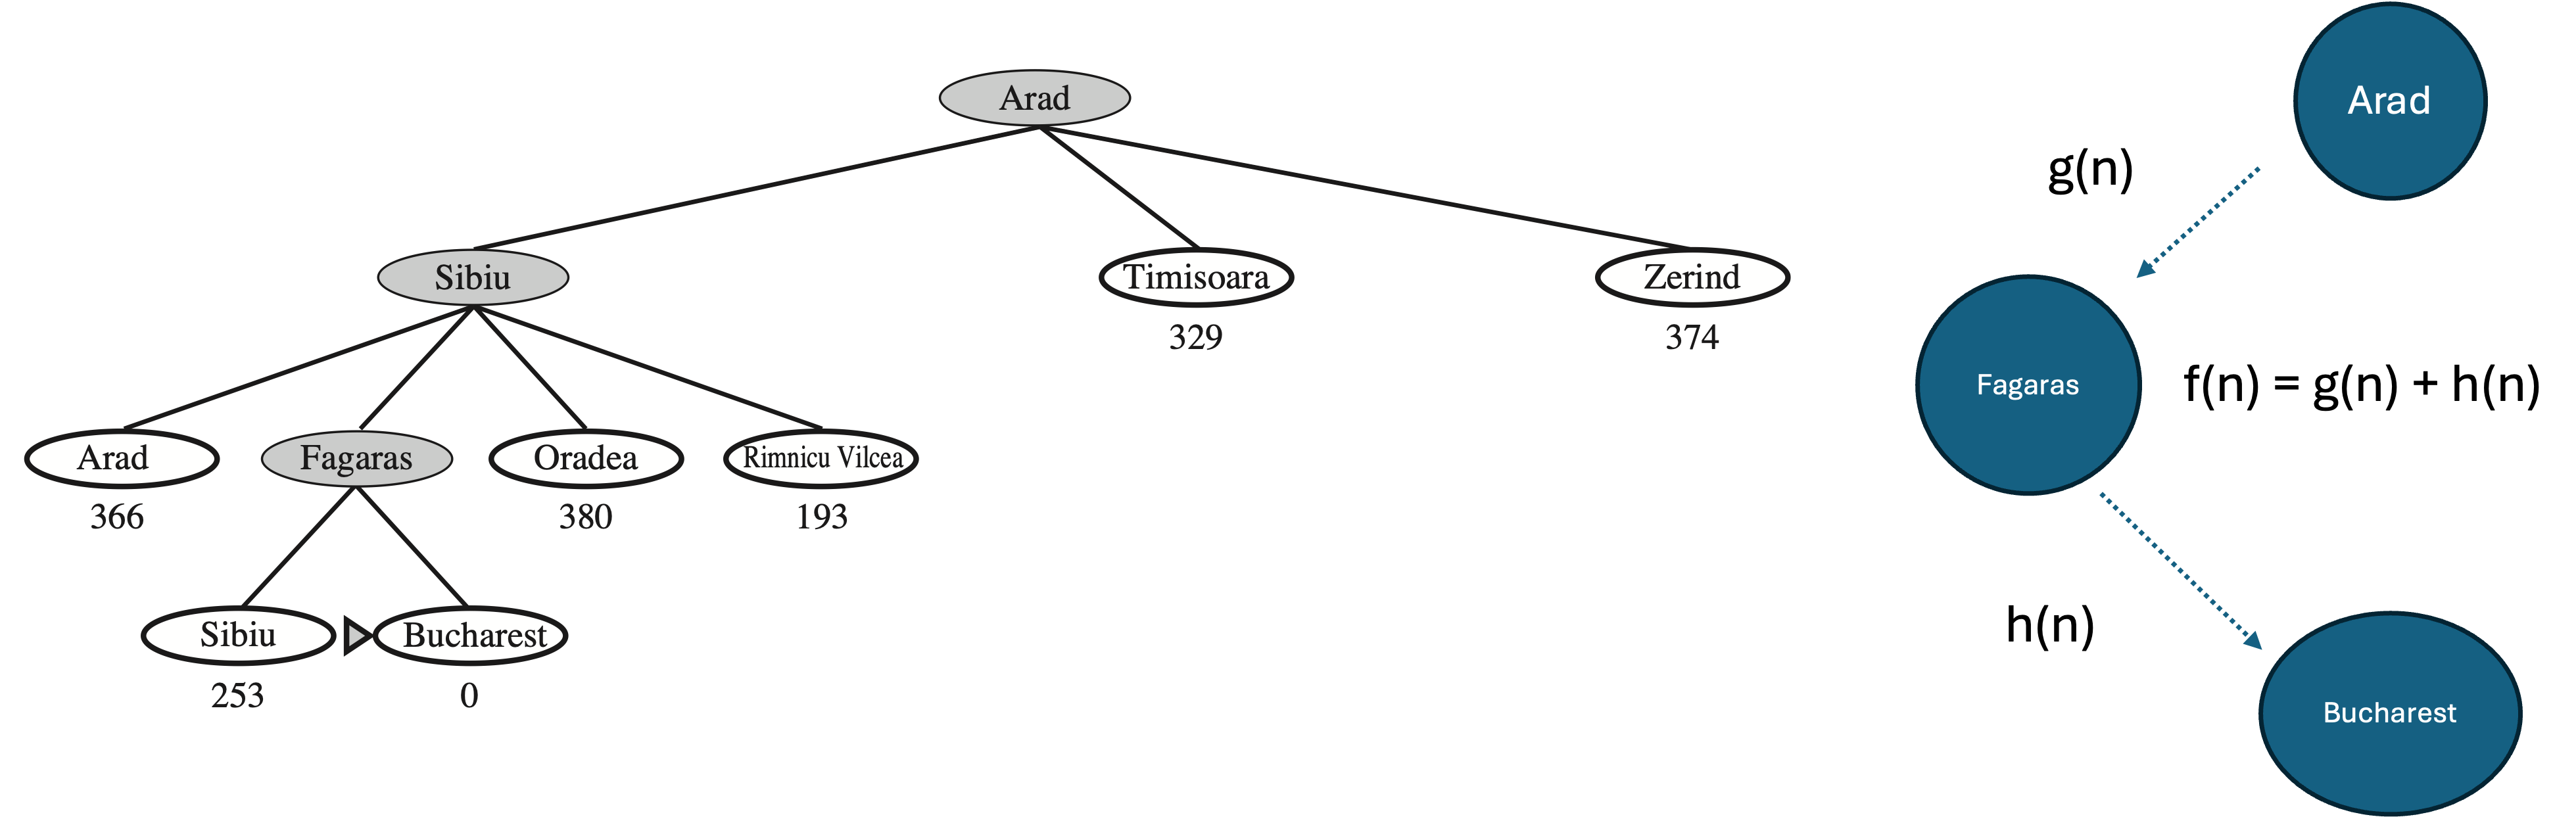
\includegraphics[scale=0.4]{./img/Afn}
\end{figure}

\end{frame} 


%%%%%%%%%%%%%%%%%%%%%%%%%%%%%%%%

\begin{frame} \frametitle{Ejemplo Búsqueda $A^*$} \small

\begin{figure}
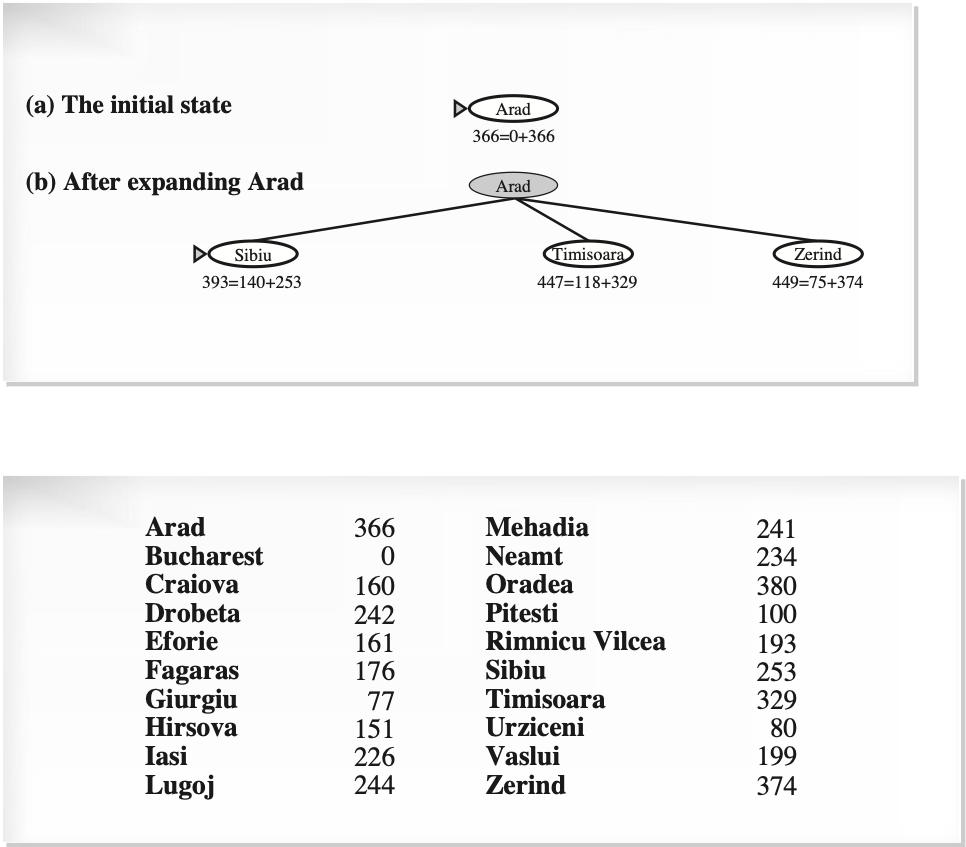
\includegraphics[scale=0.4]{./img/A1}
\end{figure}

\end{frame} 

%%%%%%%%%%%%%%%%%%%%%%%%%%%%%%%%

\begin{frame} \frametitle{Ejemplo Búsqueda $A^*$} \small

\begin{figure}
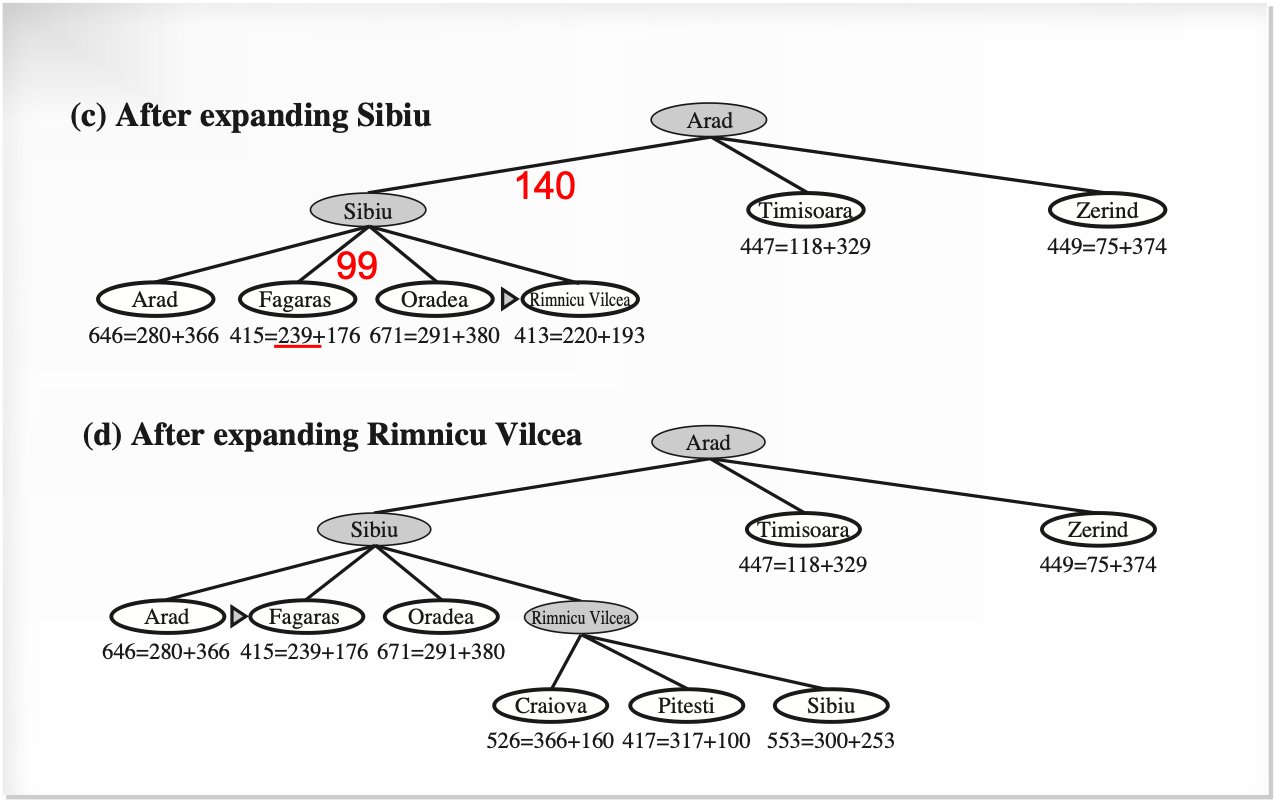
\includegraphics[scale=0.4]{./img/A2}
\end{figure}

\end{frame} 

%%%%%%%%%%%%%%%%%%%%%%%%%%%%%%%%

\begin{frame} \frametitle{Ejemplo Búsqueda $A^*$} \small

\begin{figure}
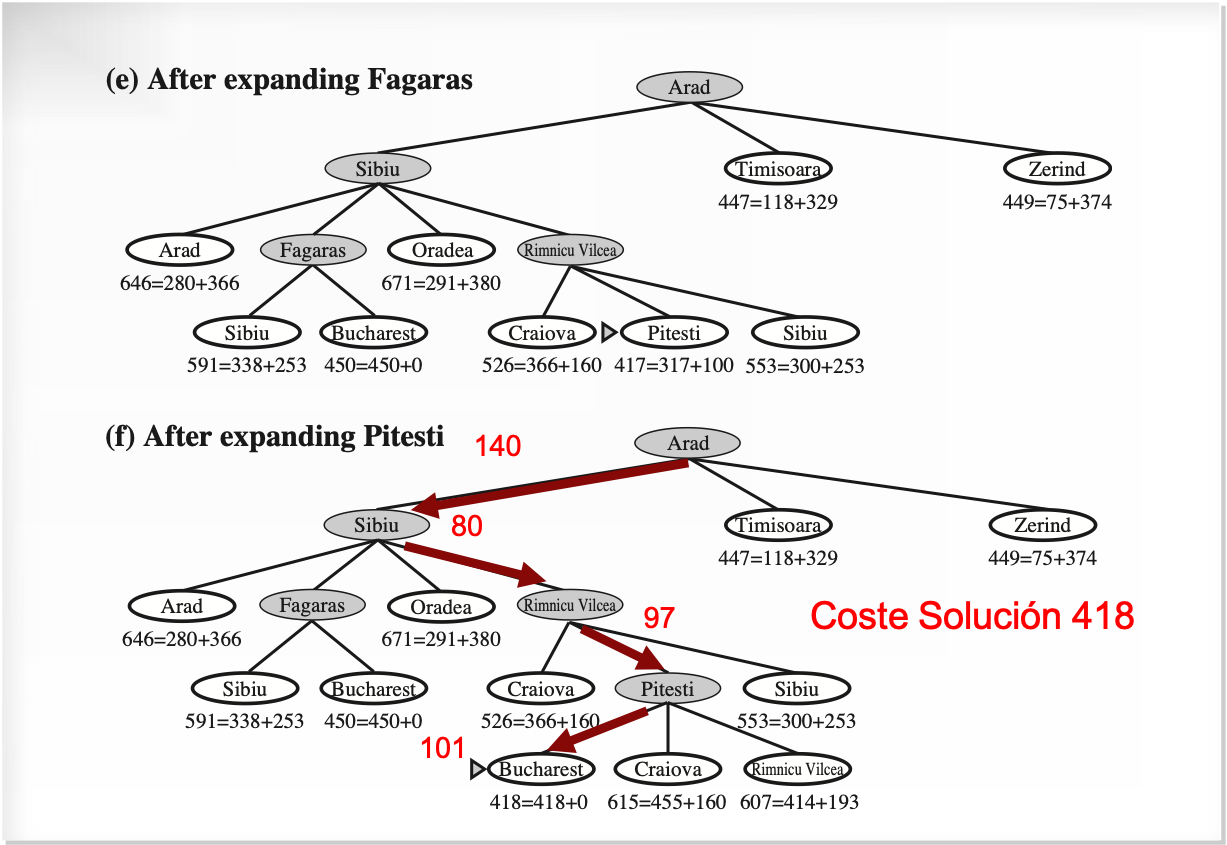
\includegraphics[scale=0.4]{./img/A3}
\end{figure}

\end{frame} 

%%%%%%%%%%%%%%%%%%%%%%%%%%%%%%%%
\begin{frame}  \frametitle{Ejecución $A^*$ }\footnotesize  

\begin{table}[]
\begin{tabular}{|l|l|l|l|}
\hline
\rowcolor[HTML]{C0C0C0} 
\textbf{Nodo seleccionado}  & \textbf{Sucesor}           & \textbf{g+h=f}               & \textbf{Orden en que se han cerrado} \\ \hline
\textbf{Arad}      & Zerind            & 75+374= 449         &                             \\ \hline
-                  & Timisoara         & 118+329= 447        &                             \\ \hline
-                  & Sibiu             & 140+253=393         & (1)                         \\ \hline\hline

\textbf{Sibiu}     & Fagaras           & (140+99)+176= 415   & (3)                         \\ \hline
-                  & Oradea            & (140+151)+380= 671  &                             \\ \hline
                   & Rimmicu           & (140+80)+193= 413   & (2)                         \\ \hline\hline

\textbf{Rimmicu}   & Pitesti           & (220+97)+100= 417   & (4)                         \\ \hline
-                  & Craiova           & (220+146)+160= 526  &                             \\ \hline\hline

\textbf{Fagaras}   & Sibiu             & -                   & cerrado                     \\ \hline
-                  & Bucharest         & (239+211)+0 = 450   & cerrado mejor               \\ \hline\hline

\textbf{Pitesti}   & Craiova           & (317+138)+160 = 615 & cerrado mejor               \\ \hline
-                  & Bucharest         & (317+101)+0 = 418   & (5)                         \\ \hline
\textbf{Bucharest} & \textbf{Solución Problema} &                     &                             \\ \hline
\end{tabular}
\end{table}

\end{frame} 


%%%%%%%%%%%%%%%%%%%%%%%%%%%%%%%%
\section{Puzzle 8}
\begin{chapter}[images/etsiinformatica4.png]{uicblue}{Problemas}
\end{chapter}



%%%%%%%%%%%%%%%%%%%%%%%%%%%%%%%%

\begin{frame} \frametitle{Problema 1- Distancias entre ciudades} \tiny

Las distancias por carretera entre las ciudades de una región vienen dadas en kilómetros en la tabla siguiente:


\begin{table}[]
\begin{tabular}{|l|l|l|l|l|l|l|l|}
\hline
  & A                                               & B                        & C                        & D                        & E                        & F                        & G                        \\ \hline
A & \cellcolor[HTML]{C0C0C0}{\color[HTML]{9B9B9B} } & 10                       & 15                       &                          &                          &                          &                          \\ \hline
B & \cellcolor[HTML]{C0C0C0}                        & \cellcolor[HTML]{C0C0C0} &                          & 5                        & 15                       &                          &                          \\ \hline
C & \cellcolor[HTML]{C0C0C0}                        & \cellcolor[HTML]{C0C0C0} & \cellcolor[HTML]{C0C0C0} &                          & 5                        & 15                       &                          \\ \hline
D & \cellcolor[HTML]{C0C0C0}                        & \cellcolor[HTML]{C0C0C0} & \cellcolor[HTML]{C0C0C0} & \cellcolor[HTML]{C0C0C0} &                          &                          & 20                       \\ \hline
E & \cellcolor[HTML]{C0C0C0}                        & \cellcolor[HTML]{C0C0C0} & \cellcolor[HTML]{C0C0C0} & \cellcolor[HTML]{C0C0C0} & \cellcolor[HTML]{C0C0C0} & 5                        & 5                        \\ \hline
F & \cellcolor[HTML]{C0C0C0}                        & \cellcolor[HTML]{C0C0C0} & \cellcolor[HTML]{C0C0C0} & \cellcolor[HTML]{C0C0C0} & \cellcolor[HTML]{C0C0C0} & \cellcolor[HTML]{C0C0C0} & 20                       \\ \hline
G & \cellcolor[HTML]{C0C0C0}                        & \cellcolor[HTML]{C0C0C0} & \cellcolor[HTML]{C0C0C0} & \cellcolor[HTML]{C0C0C0} & \cellcolor[HTML]{C0C0C0} & \cellcolor[HTML]{C0C0C0} & \cellcolor[HTML]{C0C0C0} \\ \hline
\end{tabular}
\end{table}


La siguiente tabla contiene una estimación optimista de la distancia en kilómetros desde la ciudad G a cada una de las demás ciudades:

\begin{table}[]
\begin{tabular}{|l|l|l|l|l|l|l|l|}
\hline
                    & A  & B & C & D & E & F & G \\ \hline
\textbf{Estimación} & 19 & 9 & 9 & 4 & 4 & 3 & 0 \\ \hline
\end{tabular}
\end{table}

\begin{itemize}
    \item a) Aplicar el algoritmo Greedy para encontrar un camino desde la ciudad A a la ciudad G. Indicar para cada iteración el nodo seleccionado para expansión, sus sucesores y los valores correspondientes de f(n). Mostrar el árbol de búsqueda resultante, detallando las operaciones realizadas sobre el mismo.
    \item b) Aplicar el algoritmo A* para encontrar un camino desde la ciudad A a la ciudad G. Indicar para cada iteración el nodo seleccionado para expansión, sus sucesores y los valores correspondientes de g(n), h(n) y f(n). Mostrar el árbol de búsqueda resultante, detallando las operaciones realizadas sobre el mismo.
\end{itemize}

\end{frame} 

%%%%%%%%%%%%%%%%%%%%%%%%%%%%%%%%
%%%%%%%%%%%%%%%%%%%%%%%%%%%%%%%%

\begin{frame} \frametitle{Distancias entre ciudades, Greedy} \footnotesize

\begin{table}[]
\begin{tabular}{|l|l|l|l|}
\hline
\rowcolor[HTML]{C0C0C0} 
\textbf{Nodo seleccionado}  & \textbf{Sucesor}           & \textbf{h=f}               & \textbf{Orden en que se han cerrado} \\ \hline
\textbf{A}         & B            & 9         &    (1)         \\ \hline
-                  & C            & 9        &          \\ \hline\hline

\textbf{B}     & D           & 4   & (2)          \\ \hline
-                  & E            & 4  &                \\ \hline\hline

\textbf{D}   & G             & 0                  & (3)     \\ \hline\hline

\textbf{G}   & SOLUCIÓN             & -             & -    \\ \hline

\end{tabular}
\end{table}

\end{frame} 

 
%%%%%%%%%%%%%%%%%%%%%%%%%%%%%%%%
%%%%%%%%%%%%%%%%%%%%%%%%%%%%%%%%

\begin{frame} \frametitle{Distancias entre ciudades, $A^*$} \footnotesize

\begin{table}[]
\begin{tabular}{|l|l|l|l|}
\hline
\rowcolor[HTML]{C0C0C0} 
\textbf{Nodo seleccionado}  & \textbf{Sucesor}           & \textbf{g+h=f}               & \textbf{Orden en que se han cerrado} \\ \hline
\textbf{A}         & B            & 10+ 9=19         &    (1)     \\ \hline
-                  & C            & 15+ 9=24        &     (3)     \\ \hline\hline

\textbf{B}     & D           & 15+ 4=19   & (2)          \\ \hline
-              & E          & 25 + 4 = 29  &     cerrado mejor nodo \\ \hline\hline

\textbf{D}   & G             & 35+ 0=35                 &   cerrado mejor nodo   \\ \hline\hline

\textbf{C}     & E           & 20+ 4=24   & (4)          \\ \hline
-              & F          & 30+ 3=33  &      cerrado mejor nodo          \\ \hline\hline

\textbf{E}     & F           & 25 + 3 = 28   &           \\ \hline
-              & G          & 25 + 0 = 25  &   (5)             \\ \hline\hline

\textbf{G}   & SOLUCIÓN             & -             & -    \\ \hline

\end{tabular}
\end{table}

\end{frame} 

%%%%%%%%%%%%%%%%%%%%%%%%%%%%%%%%

\begin{frame} \frametitle{Problema 2- Distancias entre ciudades} \tiny

Aplicar el algoritmo A* para hallar un camino que una las ciudades J y F. Las distancias por carretera entre las ciudades de la región vienen dadas en la tabla siguiente:


% Please add the following required packages to your document preamble:
% \usepackage[table,xcdraw]{xcolor}
% Beamer presentation requires \usepackage{colortbl} instead of \usepackage[table,xcdraw]{xcolor}
\begin{table}[]
\begin{tabular}{|c|c|c|c|c|c|c|c|c|c|c|c|}
\hline
                          & \cellcolor[HTML]{EFEFEF}{\color[HTML]{000000} A} & \cellcolor[HTML]{EFEFEF}{\color[HTML]{000000} B} & \cellcolor[HTML]{EFEFEF}{\color[HTML]{000000} C} & \cellcolor[HTML]{EFEFEF}{\color[HTML]{000000} D} & \cellcolor[HTML]{EFEFEF}{\color[HTML]{000000} E} & \cellcolor[HTML]{EFEFEF}{\color[HTML]{000000} F} & \cellcolor[HTML]{EFEFEF}{\color[HTML]{000000} G} & \cellcolor[HTML]{EFEFEF}{\color[HTML]{000000} H} & \cellcolor[HTML]{EFEFEF}{\color[HTML]{000000} I} & \cellcolor[HTML]{EFEFEF}{\color[HTML]{000000} J} & \cellcolor[HTML]{EFEFEF}{\color[HTML]{000000} K} \\ \hline
\cellcolor[HTML]{EFEFEF}A &                                                  &                                                  & 63                                               & 75                                               &                                                  & 44                                               &                                                  &                                                  &                                                  &                                                  &                                                  \\ \hline
\cellcolor[HTML]{EFEFEF}B &                                                  &                                                  & 61                                               & 77                                               &                                                  &                                                  & 64                                               &                                                  &                                                  &                                                  &                                                  \\ \hline
\cellcolor[HTML]{EFEFEF}C &                                                  &                                                  &                                                  & 29                                               &                                                  &                                                  &                                                  &                                                  &                                                  &                                                  &                                                  \\ \hline
\cellcolor[HTML]{EFEFEF}D &                                                  &                                                  &                                                  &                                                  & 38                                               &                                                  &                                                  & 56                                               &                                                  &                                                  & 34                                               \\ \hline
\cellcolor[HTML]{EFEFEF}E &                                                  &                                                  &                                                  &                                                  &                                                  & 58                                               &                                                  &                                                  &                                                  &                                                  & 59                                               \\ \hline
\cellcolor[HTML]{EFEFEF}F &                                                  &                                                  &                                                  &                                                  &                                                  &                                                  &                                                  &                                                  &                                                  &                                                  &                                                  \\ \hline
\cellcolor[HTML]{EFEFEF}G &                                                  &                                                  &                                                  &                                                  &                                                  &                                                  &                                                  & 27                                               &                                                  & 55                                               &                                                  \\ \hline
\cellcolor[HTML]{EFEFEF}H &                                                  &                                                  &                                                  &                                                  &                                                  &                                                  &                                                  &                                                  & 35                                               &                                                  & 44                                               \\ \hline
\cellcolor[HTML]{EFEFEF}I &                                                  &                                                  &                                                  &                                                  &                                                  &                                                  &                                                  &                                                  &                                                  & 40                                               &                                                  \\ \hline
\cellcolor[HTML]{EFEFEF}J &                                                  &                                                  &                                                  &                                                  &                                                  &                                                  &                                                  &                                                  &                                                  &                                                  &                                                  \\ \hline
\cellcolor[HTML]{EFEFEF}K &                                                  &                                                  &                                                  &                                                  &                                                  &                                                  &                                                  &                                                  &                                                  &                                                  &                                                  \\ \hline
\end{tabular}
\end{table}


y las distancias aéreas a la ciudad F son:


\begin{table}[]
\begin{tabular}{|c|c|c|c|c|c|c|c|c|c|c|c|}
\hline
                                   & \cellcolor[HTML]{C0C0C0}\textbf{A} & \cellcolor[HTML]{C0C0C0}\textbf{B} & \cellcolor[HTML]{C0C0C0}\textbf{C} & \cellcolor[HTML]{C0C0C0}\textbf{D} & \cellcolor[HTML]{C0C0C0}\textbf{E} & \cellcolor[HTML]{C0C0C0}\textbf{F} & \cellcolor[HTML]{C0C0C0}\textbf{G} & \cellcolor[HTML]{C0C0C0}\textbf{H} & \cellcolor[HTML]{C0C0C0}\textbf{I} & \cellcolor[HTML]{C0C0C0}\textbf{J} & \cellcolor[HTML]{C0C0C0}\textbf{K} \\ \hline
\cellcolor[HTML]{C0C0C0}\textbf{F} & 38                                 & 97                                 & 59                                 & 62                                 & 46                                 &                                    & 111                                & 112                                & 139                                & 158                                & 87                                 \\ \hline
\end{tabular}
\end{table}

Mostrar el árbol de búsqueda resultante, y detallar en cada paso el nodo seleccionado, así como los valores de g(n), h(n) y f(n) de los nodos generados.

\end{frame} 


%%%%%%%%%%%%%%%%%%%%%%%%%%%%%%%%
\begin{frame} [fragile ]\frametitle{Puzzle 8 - Heurístico} \footnotesize

\begin{columns}

\begin{column}{0.5\textwidth}  


h(n) = número de piezas mal colocadas.



\begin{figure}
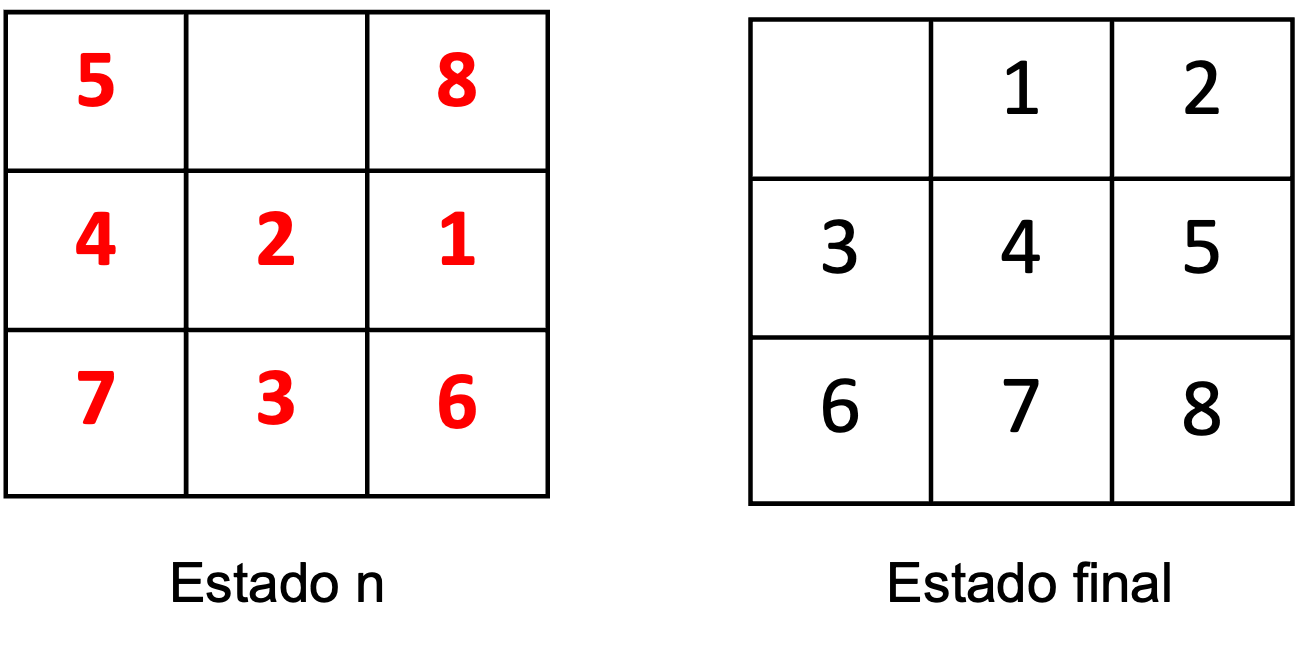
\includegraphics[scale=0.4]{./img/Puzzle8Malcolocadas}
\end{figure}

h(n) = 8

\end{column}

\begin{column}{0.5\textwidth}\scriptsize

h(n) = distancia (manhattan) de cada posición a su posición objetivo.

\begin{figure}
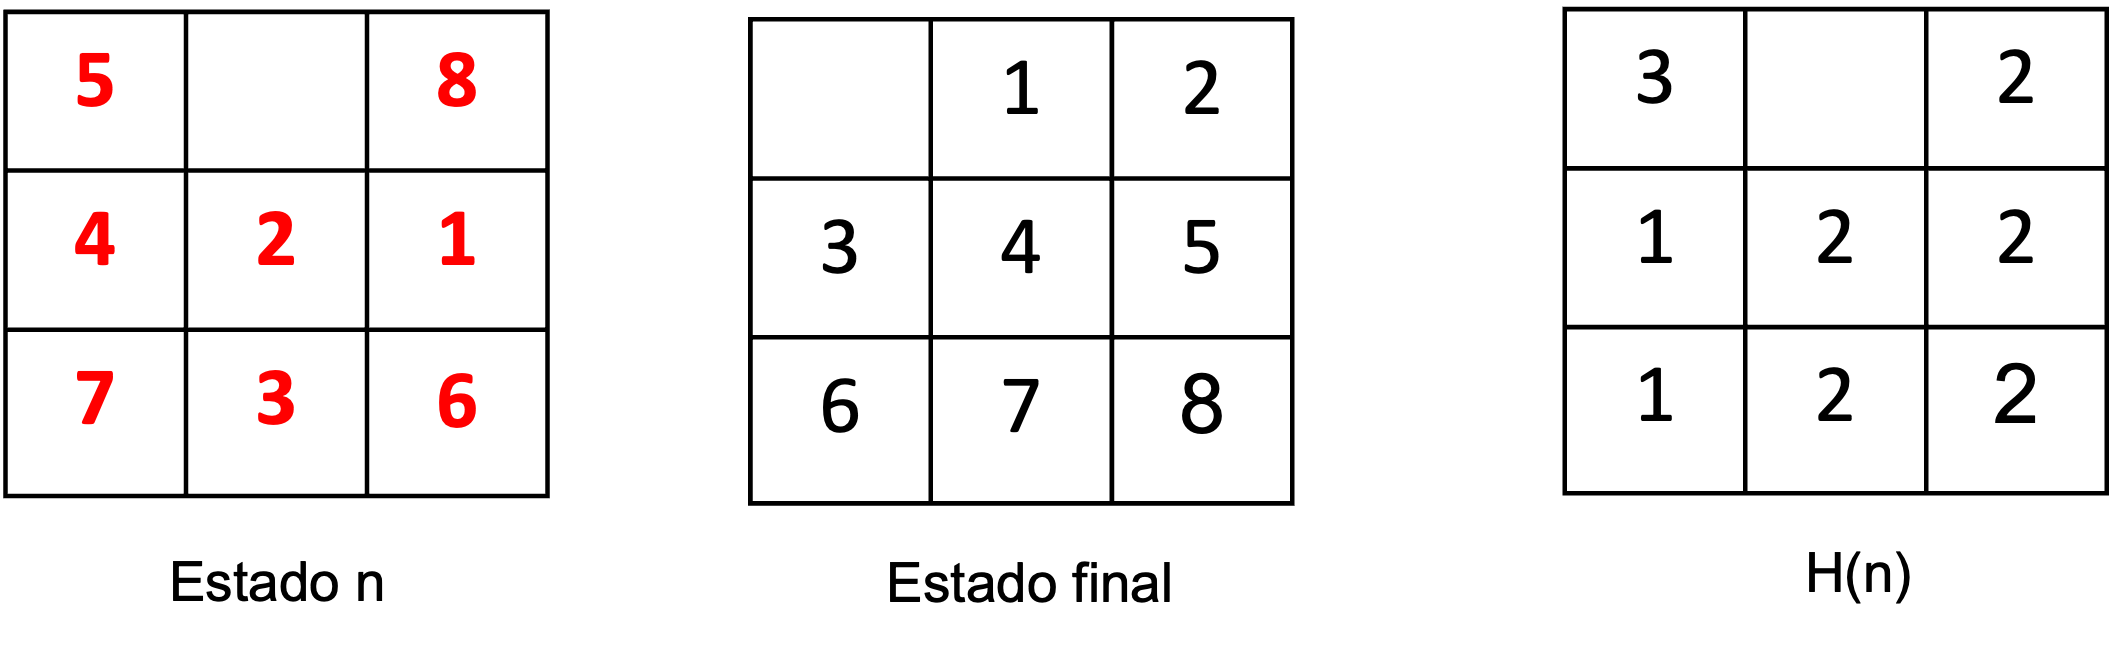
\includegraphics[scale=0.4]{./img/Puzzle8Manhattam}
\end{figure}

h(n) = 15
\end{column}

\end{columns}


\end{frame} 

%%%%%%%%%%%%%%%%%%%%%%%%%%%%%%%%
%\begin{frame} [fragile ]\frametitle{Puzzle 8 - Heurístico} \footnotesize
%\begin{minted}[fontsize=\small]{python}

%initial_state = '1'
%goal_state = '8'
%problem = ProblemGrafo(initial_state, goal_state)
%solution_node = depth_first_search(problem)
%\end{minted}

%\end{frame} 







%%%%%%%%%%%%%%%%%%%%%%%%%%%%%%%%
%\begin{frame}  \small  
%\end{frame} 


%%%%%%%%%%%%%%%%%%%%%%%%%%%%%%%%
%\begin{frame}  \small  
%\end{frame} 


%%%%%%%%%%%%%%%%%%%%%%%%%%%%%%%%
%\begin{frame}  \small  
%\end{frame} 

%%%%%%%%%%%%%%%%%%%%%%%%%%%%%%%%
%%%%%%%%%%%%%%%%%%%%%%%%%%%%%%%%

%%%%%%%%%%%%%%%%%%%%%%%%%%%%%%%%
%%%%%%%%%%%%%%%%%%%%%%%%%%%%%%%%
   
\backmatter


\end{document}